%invertedCurve
There have been 17 years when there was at least one week with an inverted yield curve: 1927, 1928, 1929 1930, 1959, 1966, 1967, 1968, 1969, 1970, 1973, 1974, 1979, 1980, 1981, 2000, and 2006.\cite{Shaw}  Most of those years were associated with tough times in the United States economy. It is generally held that a prolonged inverted yield curve produces a subsequent recession.\cite{Shaw}  The rule of thumb is that an inverted yield curve (short rates above long rates) indicates a recession in about a year, and yield curve inversions have preceded each of the last seven recessions.\cite{Haubrich}  Monetary policy has a significant influence on the yield curve spread and hence on real activity over the next several quarters.\cite{Estrella2} A rise in the short rate tends to flatten the yield curve as well as to slow real growth in the near term.  The federal funds rate is a simple monetary policy tool that can greatly influence the yield curve.

\begin{figure}[H]
\centering
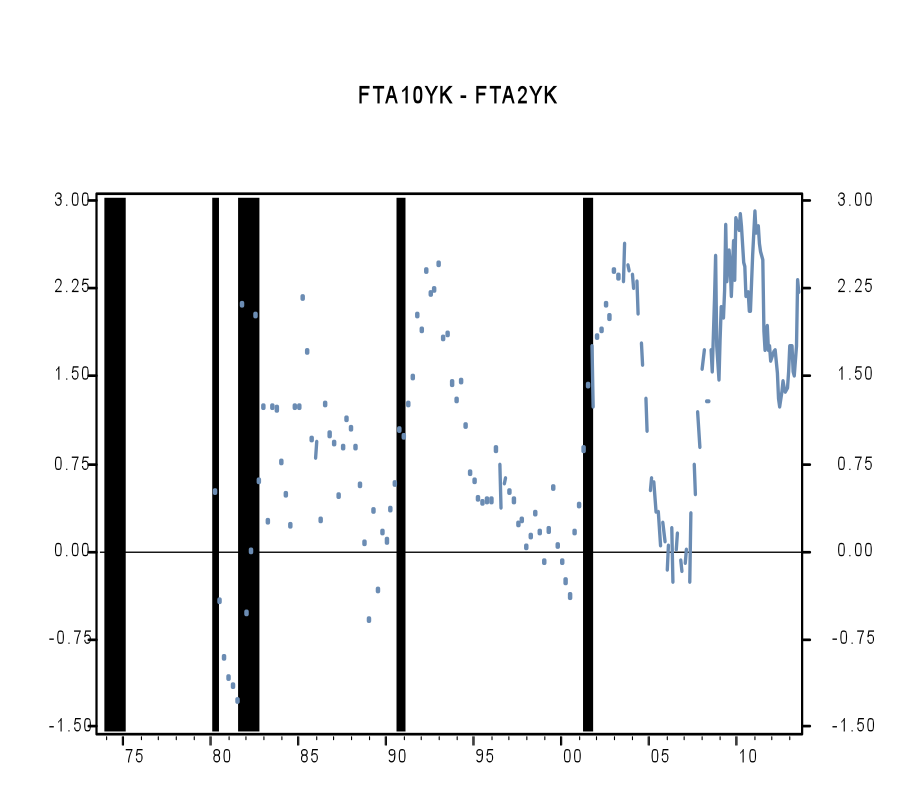
\includegraphics[scale=.70]{figure/InvertedTbill.png}\\[-0.7cm]
\caption{Inverted Treasury Yields: 2 Year and 10 Year\label{fig:inverted}}
\end{figure}

Forecasting recession with the yield curve is quick and simple.  Pinpointing the exact cause and severity of recession, requires consideration of more macroeconomic indicators.  A simple financial indicator such as the yield curve can be used to double-check both econometric and judgmental predictions, aligning heuristic analysis with indicators of greater detail.  For example, if forecasts from an econometric model and the yield curve agree, confidence in the model?s results can be enhanced.\cite{Estrella2}

%%%%%%%%%%%%%%%%%%%%%%%%%%%%%%%%%%%%%
\subsection{Ripple Effects from Treasury Market}
The treasury bill is considered a risk-free asset and is consistently used as the base rate for many fixed income securities.  The corporate bond market and the municipal bond market are both intimately related to the rates in the treasury market.  Additionally, the maturity that corresponds to a particular treasury rate, is widely used as a predictor of future economic inflation.

\begin{figure}[H]
\centering
\begin{subfigure}{.5\textwidth}
  \centering
  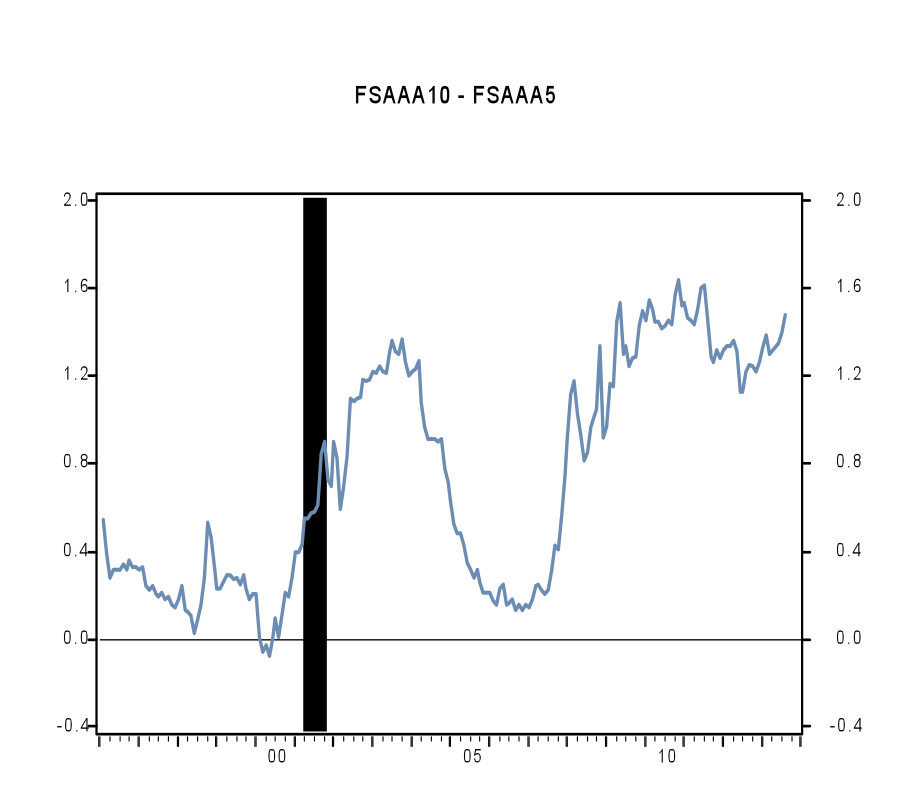
\includegraphics[width=1.0\linewidth]{figure/Corp10Year_5Year.png}
  \caption{AAA Rated Corporate Debt}
  \label{fig:corp}
\end{subfigure}%
\begin{subfigure}{.5\textwidth}
  \centering
  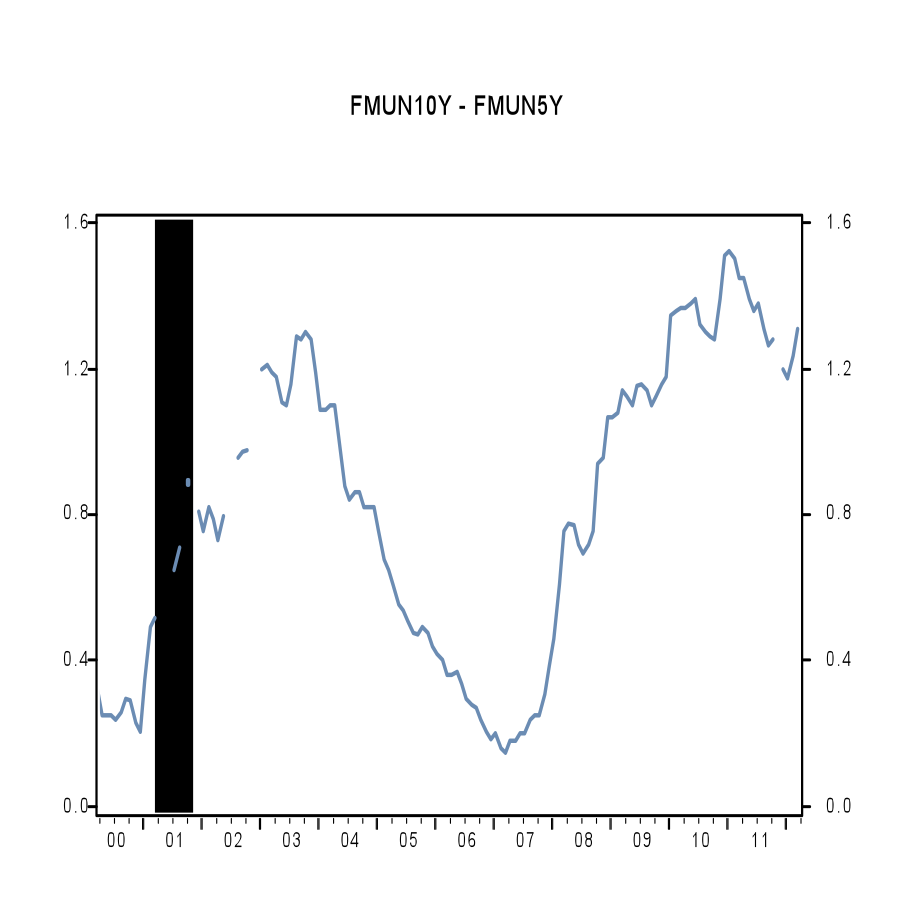
\includegraphics[width=0.9\linewidth]{figure/NewMuni.png}
  \caption{Municipal Debt}
  \label{fig:muni}
\end{subfigure}
\caption{Yield Curves: 5 Year and 10 Year Spread}
\label{fig:ripple}
\end{figure}

In figure\ref{fig:ripple} the flattening spread between corporate AAA rated bonds and municipal bonds of 5 and 10 years occurs in the same period as the treasury curve inversion.  The treasury spread is a great recession indicator because its inversion is tied closely to the present liquidity risk, and from this liquiditiy risk presumably is the factor that penetrates into the corporate and municipal bond markets.\cite{Gallmeyer}